In this section, a moving boundary problem will be presented 
in order to show the ALE description functionality. 
The mesh was moved according to Eq. \ref{mesh velocity eq}, 
whereas the boundary will be moved by the pulsating equation:

\begin{equation} \label{boundary top}
y_{\Gamma} = 2A\sin\left(kx\rigth)\cos\left(wt\right)
\end{equation}


\medskip
\noindent
where, 
$y_{\Gamma}$ is the top and bottom boundaries,
$A$ is the wave amplitude,
$k$ is the wavenumber,
$x$ is the horizontal coordinate,
$w$ is the angular frequency and
$t$ is the time variable.

\medskip
The \ref{moving boundary fig} shows a cycle of the boundary movement, 
tending to its maximum expansion and contraction. 
As mentioned in section \ref{laplacian smoothing}, 
the use of the Laplacian smoothing method becomes 
essential for the simulation to be performed.


\begin{figure}[H]
     \begin{minipage}{.50\linewidth}
      \centering
      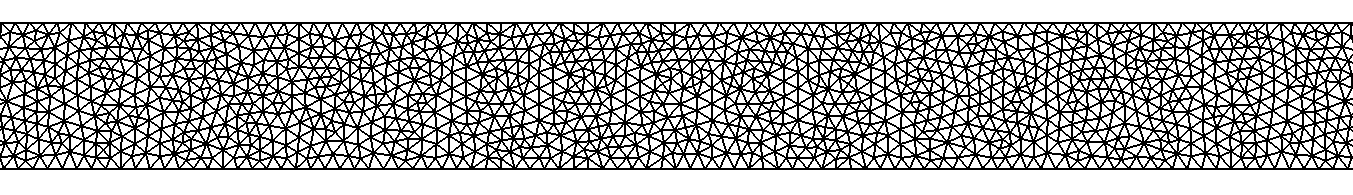
\includegraphics[scale=0.16]{./02_chaps/cap_validation/figure/comp0.png}\\
     \end{minipage}%
     \begin{minipage}{.50\linewidth}
      \centering
      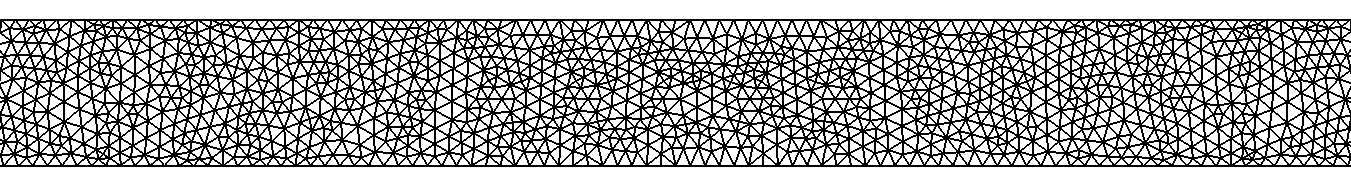
\includegraphics[scale=0.16]{./02_chaps/cap_validation/figure/ext0.png}\\
     \end{minipage}
     \begin{minipage}{.50\linewidth}
     \medskip
      \centering
      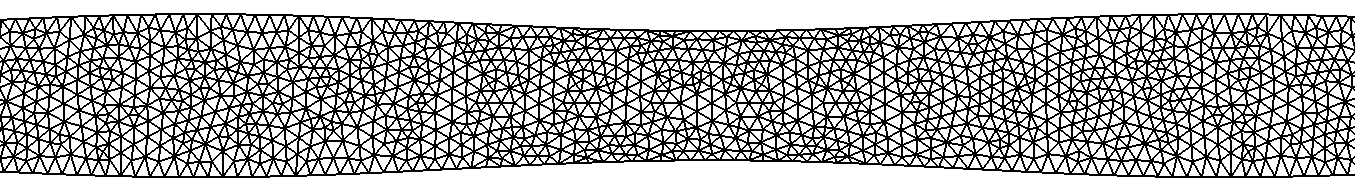
\includegraphics[scale=0.16]{./02_chaps/cap_validation/figure/comp1.png}\\
     \end{minipage}%
     \begin{minipage}{.50\linewidth}
     \medskip
      \centering
      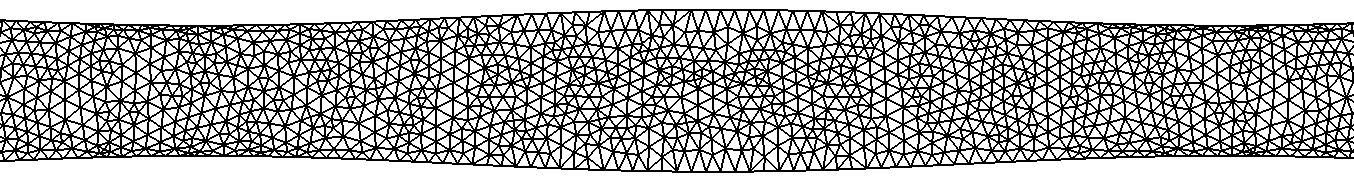
\includegraphics[scale=0.16]{./02_chaps/cap_validation/figure/ext1.png}\\
     \end{minipage}\\[7pt]
     \begin{minipage}{.50\linewidth}
      \centering
      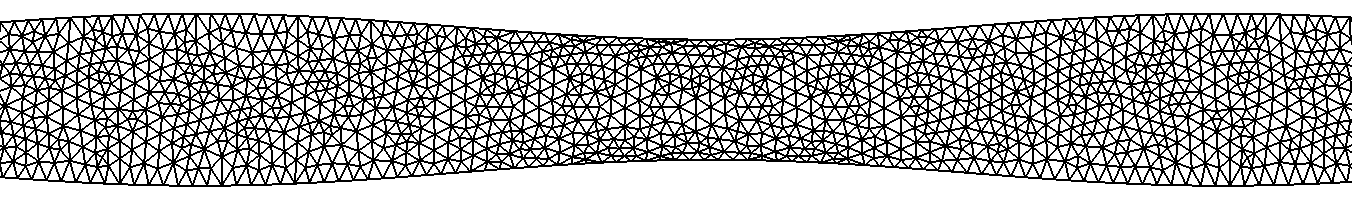
\includegraphics[scale=0.16]{./02_chaps/cap_validation/figure/comp2.png}\\
     \end{minipage}%
     \begin{minipage}{.50\linewidth}
      \centering
      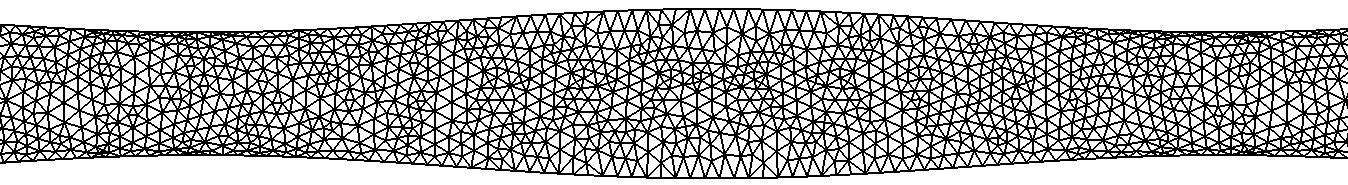
\includegraphics[scale=0.16]{./02_chaps/cap_validation/figure/ext2.png}\\
     \end{minipage}
     \begin{minipage}{.50\linewidth}
     \medskip
      \centering
      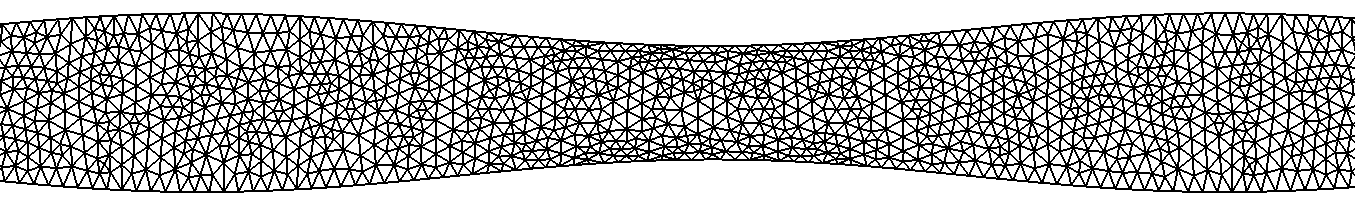
\includegraphics[scale=0.16]{./02_chaps/cap_validation/figure/comp3.png}\\
     (a)
     \end{minipage}%
     \begin{minipage}{.50\linewidth}
     \medskip
      \centering
      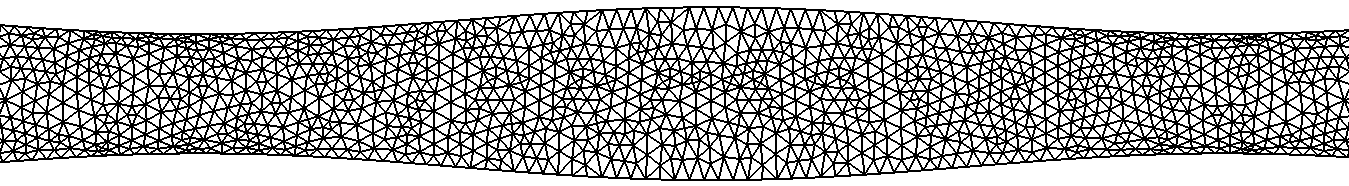
\includegraphics[scale=0.16]{./02_chaps/cap_validation/figure/ext3.png}\\
     (b)
     \end{minipage}
     \medskip
     \caption{
The moving boundary problem tending to  
     (a) maximum contraction and
     (b) maximum expansion
in the middle of channel.
}
     \label{moving boundary fig}
\end{figure}




\medskip
The \ref{contraction velocity} shows the comparison between the 
numerical and analytical solution for the maximum contraction 
of the channel. Whereas the \ref{expansion velocity} 
shows the comparison between the solutions for 
the maximum expansion of the channel.

\begin{figure}[H]
     \centering
     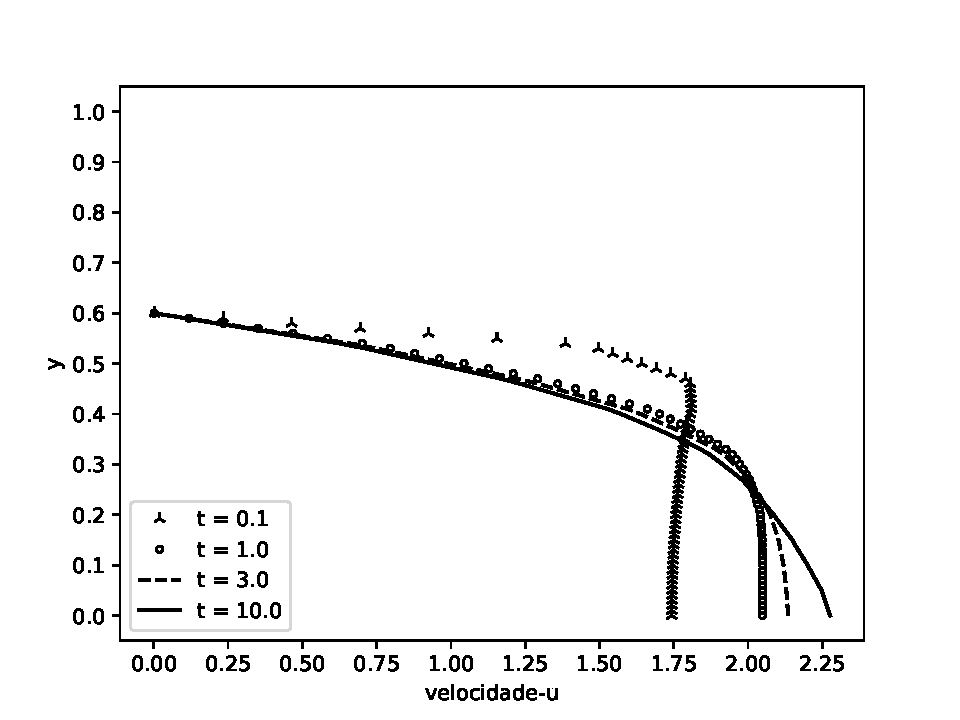
\includegraphics[scale=1]{./02_chaps/cap_solution/figure/vel_Curved_evol.pdf}\\
     \caption{The unsteady velocity profile for the curved channel.}
     \label{contraction velocity}
\end{figure}


\begin{figure}[H]
     \centering
     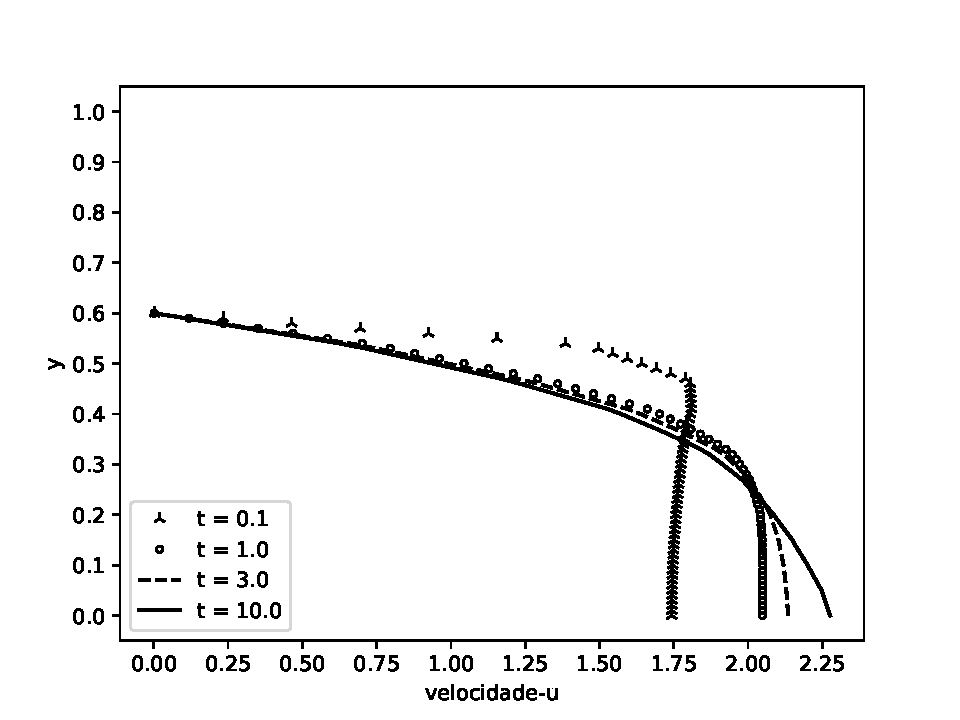
\includegraphics[scale=1]{./02_chaps/cap_solution/figure/vel_Curved_evol.pdf}\\
     \caption{The unsteady velocity profile for the curved channel.}
     \label{expansion velocity}
\end{figure}




\newpage
